\documentclass{article}

\usepackage{graphicx}

\title{Homework 1}
\author{Mitchel Fields}
\begin{document}

\maketitle
\begin{itemize}

	\item [\textbf{2.2}]
	\begin{itemize}
		\item [\textbf{(b)}] $(x + y) (x + \overline{y}) = x(y + \overline{y}) = x(1) = x$
		\item [\textbf{(c)}] $xyz + \overline{x}y + xy\overline{z} = y(xz + \overline{x} + x\overline{z}) = y(\overline{x} + x(z + \overline{z})) = y(\overline{x} + x(1)) = y(1) = y$
		\item [\textbf{(d)}] $(A + B)(\overline{A} + \overline{B}) = (A + B)\overline{(AB)} = A\overline{B} + \overline{A}B = A \oplus B$
		\item [\textbf{(e)}] $(a + b + \overline{c})(\overline{a}.\overline{b} + c) = (a + b + \overline{c})(\overline{a + b} + c) = (a + b) \oplus c$
		\item [\textbf{(f)}] $\overline{a}bc + ab\overline{c} + abc + \overline{a}b\overline{c} = b(\overline{a}c + a\overline{c} + ac + \overline{a}\overline{c}) = b(1) = b$
	\end{itemize}

	\item [\textbf{2.10}]
	\begin{itemize}
		\item [\textbf{(a)}] The Boolean function $E = F_1 + F_2$ is true when either $F_1$ or $F_2$ or both are true. Thus it contains the union of their minterm sets.
		\item [\textbf{(b)}] The Boolean function $G = F_1F_2$ is true only when both $F_1$ and $F_2$ are true. Thus it contains the intersection of their minterm sets.
	\end{itemize}

	\item [\textbf{2.11}]
	\begin{itemize}
		\item [\textbf{(a)}] $F = xy + x\overline{y} + \overline{y}z$\\
		\begin{tabular}{c | c | c | c | c | c | c}
		$x$ & $y$ & $z$ & $xy$ & $x\overline{y}$ & $\overline{y}z$ & $xy + x\overline{y} + \overline{y}z$\\ \hline
		$0$ & $0$ & $0$ & $0$ & $0$ & $0$ & $0$ \\
		$0$ & $0$ & $1$ & $0$ & $0$ & $1$ & $1$ \\
		$0$ & $1$ & $0$ & $0$ & $0$ & $0$ & $0$ \\
		$0$ & $1$ & $1$ & $0$ & $0$ & $0$ & $0$ \\
		$1$ & $0$ & $0$ & $0$ & $1$ & $0$ & $1$ \\
		$1$ & $0$ & $1$ & $0$ & $1$ & $1$ & $1$ \\
		$1$ & $1$ & $0$ & $1$ & $0$ & $0$ & $1$ \\
		$1$ & $1$ & $1$ & $1$ & $0$ & $0$ & $1$ \\
		\end{tabular}
		\item [\textbf{(b)}] $F = bc + \overline{a}.\overline{c}$\\
		\begin{tabular}{c | c | c | c | c | c}
		$a$ & $b$ & $c$ & $bc$ & $\overline{a}.\overline{c}$ & $bc + \overline{a}.\overline{c}$\\ \hline
		$0$ & $0$ & $0$ & $0$ & $1$ & $1$ \\
		$0$ & $0$ & $1$ & $0$ & $0$ & $0$ \\
		$0$ & $1$ & $0$ & $0$ & $1$ & $1$ \\
		$0$ & $1$ & $1$ & $1$ & $0$ & $1$ \\
		$1$ & $0$ & $0$ & $0$ & $0$ & $0$ \\
		$1$ & $0$ & $1$ & $0$ & $0$ & $0$ \\
		$1$ & $1$ & $0$ & $0$ & $0$ & $0$ \\
		$1$ & $1$ & $1$ & $1$ & $0$ & $1$ \\
		\end{tabular}
	\end{itemize}

	\item [\textbf{2.14}]
	\begin{itemize}
		\item [\textbf{(a)}] With AND, OR, and inverter gates\\
		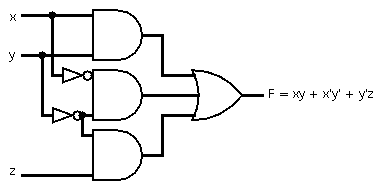
\includegraphics{214a}
		\item [\textbf{(b)}] With OR and inverter gates\\
		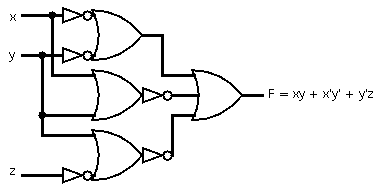
\includegraphics{214b}
		\item [\textbf{(c)}] With AND and inverter gates\\
		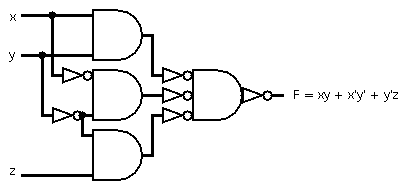
\includegraphics{214c}
	\end{itemize}

	\item [\textbf{Homework Problem}] Write a Python or Java program (whichever language is easier for you to use), to generate the truth table of the function F3 of Figure 2.4 in Mano.

\end{itemize}

	
\end{document}